% Style for a MSc paper at Warsaw School of Economics
% Michał Ramsza
% Friday, December 14, 2012

% --- document class and other global stuff ---------------------------
\documentclass[polish, twoside, 12pt, a4paper]{article}

%% --- packages --------------------------------------------------------
\usepackage{textcomp}
\usepackage{times}
\usepackage{amsmath}
\usepackage{amsfonts}
\usepackage{amssymb}
\usepackage{amsthm}
\usepackage[T1]{fontenc}
\usepackage[utf8]{inputenc}
\usepackage{graphicx}
\usepackage{xcolor}
\usepackage{enumitem}
\usepackage[polish]{babel}
\usepackage[centering, left=3.5cm, right=2.5cm, textheight=24cm]{geometry}

% --- packages for citations ------------------------------------------
\usepackage{natbib}
\AtBeginDocument{\renewcommand{\harvardand}{i}}

% --- package for automatic insertion of R code -----------------------
\usepackage{listings}
\lstset{language=R,%
   numbers=left,%
   tabsize=3,%
   numberstyle=\footnotesize,%
   basicstyle=\ttfamily \footnotesize \color{black},%
   escapeinside={(*@}{@*)}}

% --- support for links -----------------------------------------------
\usepackage{url}
\usepackage{hyperref}
\hypersetup{colorlinks=true,
            linkcolor=black,
            citecolor=darkgray,
            urlcolor=darkgray,
            pagecolor=darkgray}

% --- support for large tables and other stuff ------------------------
\usepackage{longtable}
% \usepackage{subfigure} % this package will not work with subcaption package
\usepackage{float}
\usepackage{caption}
\usepackage{subcaption}
\usepackage{wrapfig}
\usepackage{pdflscape} % relevant for wide tables (rotating pages)

% --- packages for game theory -----------------------------------------
\usepackage{sgame}

% --- support for no widows --------------------------------------------
\usepackage[defaultlines=4,all]{nowidow}

% --- quotation for polish language \enquote{}
\usepackage[autostyle]{csquotes}
\DeclareQuoteAlias{dutch}{polish}

% --- definitions for environments -------------------------------------
\theoremstyle{definition}
    \newtheorem{condition}{Założenie}
    \newtheorem{example}{Przykład}

\theoremstyle{plain}
    \newtheorem{definition}{Definicja}
    \newtheorem{proposition}{Stwierdzenie}
    \newtheorem{theorem}{Twierdzenie}
    \newtheorem{cor}{Wniosek}

\theoremstyle{remark}
    \newtheorem{remark}{Uwaga}

% --- other settings --------------------------------------------------
\linespread{1.5}
\frenchspacing
\sloppy
\allowdisplaybreaks[4]
\raggedbottom
\clubpenalty=10000
\widowpenalty=10000

% --- only if required ------------------------------------------------
\AtBeginDocument{\renewcommand*{\figurename}{Wykres}}
\AtBeginDocument{\renewcommand*{\tablename}{Tabela}}

% --- changing definition of footnote ---------------------------------
\makeatletter
\renewcommand\footnotesize{%
   \@setfontsize\footnotesize\@ixpt{10}%
   \abovedisplayskip 8\p@ \@plus2\p@ \@minus4\p@
   \abovedisplayshortskip \z@ \@plus\p@
   \belowdisplayshortskip 4\p@ \@plus2\p@ \@minus2\p@
   \def\@listi{\leftmargin\leftmargini
               \topsep 4\p@ \@plus2\p@ \@minus2\p@
               \parsep 2\p@ \@plus\p@ \@minus\p@
               \itemsep \parsep}%
   \belowdisplayskip \abovedisplayskip
}
\makeatother


% ---------------------------------------------------------------------
\begin{document}

% --- strona tytulowa -------------------------------------------------
\begin{titlepage}
\centering


\includegraphics[width=0.66\textwidth]{logo.JPG}

\vspace*{0.5cm}
Studium magisterskie\\
\begin{flushleft}
Kierunek: Metody Ilościowe w Ekonomii i Systemy Informacyjne\\
%Specjalność: <specjalność>
% Forma studiów: <forma studiów (stacjonarne, itd.)>
\end{flushleft}

\vspace*{.5cm}
\rule{0cm}{1cm}\hfill
\begin{minipage}{9cm}
Imie i nazwisko autora: Oskar Furmańczuk\\
Nr albumu: 81794
\end{minipage}

\vspace*{1cm}
\begin{minipage}{12cm}
\centering
\Large
\textbf{Wpływ tweetów na amerykański indeks giełdowy SP 500. Analiza z wykorzystaniem metod uczenia maszynowego.}
\end{minipage}

\vspace*{2cm}
\rule{0cm}{1cm}\hfill
\begin{minipage}{9cm}
Praca licencjacka napisana\\
w Katedrze Matematyki i Ekonomii Matematycznej\\
pod kierunkiem naukowym\\
dr hab. Michała Ramszy
\end{minipage}

\vfill
Warszawa 2021
\end{titlepage}

\rule{1ex}{0ex}\clearpage


% --- table of contents -----------------------------------------------
\cleardoublepage
\tableofcontents

% --- chapter ---------------------------------------------------------
\cleardoublepage
\section{Wprowdzenie}

Formatka dla pracy licencjackiej w Szkole Głównej Handlowej.

% --- chapter ---------------------------------------------------------
\clearpage
\section{Rzeczy podstawowe}

Tutaj zawsze pojawia się krótkie streszzcenie tego co jest w tym rozdziale.

\subsection{Kompilowanie plików \LaTeX}

Plik  \verb+.tex+ jest zwykłym plikiem tekstowym. Plik ten zawiera treść oraz komendy formatujące \LaTeX'a.Aby otrzymać dokument w formacie \verb+.pdf+ należy skompilować plik \verb+.tex+ używając następującej sekwencji \verb+pdflatex+, \verb+biblatex+, \verb+pdflatex+, \verb+pdflatex+. Jest to typowa sekwencja często podpięta pod jeden przycisk lub skrót klawiaturowy w edytorach przystosowanych do pracy z \LaTeX'em.

\subsection{Podstawowe formatowanie tekstu}

Paragrafy są kodowane poprzez zostawienie pustej linii. Aby rozpocząć nowy paragraf należy zostawić pustą linię. Przykładowo:
\begin{verbatim}
This is the first paragraph.

This is the next paragraph.
\end{verbatim}

Wszystko dotyczące paragrafu, typu wcięcia, odstępy itd. są formatowane automatycznie, nie ma potrzeby zajmowania się tym ręcznie.

Podstawowe formatowanie typu: pogrubienie, italic itd. otrzymuje się komendami: \verb+\textbf{}+, \verb+\textit{}+, \verb+\underline{}+, dającymi \textbf{text}, \textit{text}, \underline{text}. Cytowanie wykonujemy przez zastosowanie \verb+\enquote{}+ co daje \enquote{efekt}.

Ułożenie tekstu (podstawowe) można otrzymać używając otoczeń \verb+center+, \verb+flushleft+ i \verb+\flushright+. Przykłady:

\begin{center}
  This is centered.
\end{center}

\begin{flushleft}
  This is aligned to the left.
\end{flushleft}

\begin{flushright}
  This is aligned to the right.
\end{flushright}

W ramach innego otoczenia, np. \verb+table+ czy \verb+figure+ można użyć komendy \verb+\centering+.

\subsection{Czcionka i jej wielkość}

Technicznie można użyć prawie dowolnej czcionki i dowolnie zmienić jej wielkość. Nie robią Państwo tego.

% --- chapter ---------------------------------------------------------
\clearpage
\section{Matematyka}

Tutaj zawsze pojawia się krótkie streszzcenie tego co jest w tym rozdziale\footnote{To jest testowanie co się dzieje z rzeczami w odnośnikach dolnych. Tutaj też możemy wstawić matematykę \( x^2 - f(x) = g(x) \) aczkolwiek to nie jest zachowanie, które jest polecane. Można również wstawić URL do strony, co jest zachowaniem typowym: \url{https://tex.stackexchange.com/questions/249415/set-font-size-for-footnotes}.}.

\subsection{Podstawowa matematyka}

W dokumencie \LaTeX'owym mamy dwa rodzaje matematyki. Pierwszy jest wewnątrz linii a drugi jest wycentrowany. Typowy przykład dla matematyki w lini to  \( F(x) = \int_{-\infty}^{x} f(\omega) d\omega \) z kodem wyglądającym w następujący sposób: \verb!\( F(x) = \int_{-\infty}^{x} f(\omega) d\omega \)!. Matematyka wycentrowana wygląda w następujący sposób
\[
F(x) = \int_{-\infty}^{x} f(\omega) d\omega
\]
z kodem postaci
\begin{verbatim}
\[
F(x) = \int_{-\infty}^{x} f(\omega) d\omega
\]
\end{verbatim}
Jak Państwo widzą ten sam wzór jest składany inaczej zależnie od miejsca znajdowania się.

\subsection{Odnośniki do matematyki i innych rzeczy}

Aby można było odnieść się do wzoru to musi być on wycentrowany i podany wewnątrz otoczenia \verb+equation+. Wewnątrz tego otoczenia należy podać komendę \verb+\label{}+. Odnośnik do równania budujemy poprzez komendę \verb+\ref{}+. Przykład
\begin{equation}
\label{eq:this-is-very-important-equation}
F(x) = \int_{-\infty}^{x} f(\omega) d\omega.
\end{equation}
Aby odnieść się do powyższego równania używamy komendy \verb+\ref{}+ co produkuje (\ref{eq:this-is-very-important-equation}). Para \verb+\label{}+ / \verb+\ref{}+ działa dla wsystkich rodzajów odnośników.

\subsection{Nieco bardziej skomplikowane formuły}

Tutaj przykład nieco bardziej skomplikowanego wzoru. Niech \( A  \) będzie macierzą
\[
A =
\left(
\begin{bmatrix}
1                   & \alpha^2                             \\
2                   & \sqrt{\pi} - \log(x-\sin(y))
\end{bmatrix}^{2}
-
\begin{bmatrix}
1                   & f(x)                                 \\
2                   & g(y)
\end{bmatrix}
\cdot
\begin{bmatrix}
x                                                          \\
y
\end{bmatrix}
\right),
\]
gdzie
\[
f(x) =
\left\{
  \begin{aligned}
    \frac{1}{x}     & \quad \text{dla \(x<-\frac{1}{2}\),} \\
    \frac{1}{1+x^2} & \quad \text{dla \(x \geq -\frac{1}{2}\)}
  \end{aligned}
\right.
\]
oraz
\[
g(y) = \sin\left(\frac{\mathrm{\mathbf{E}}(X)}{\cos(y) + \log(y)}\right),
\quad\text{gdzie \( X \sim \mathrm{N}(0, \sigma)  \).}
\]

Bardzo łatwo można składać gry w postaci normalnlej. Poniżej przykład takiej gry.

\begin{game}{3}{3}
    & $L$    & $M$    & $H$    \\
$L$ & $16,9$ & $3,13$ & $0,3$  \\
$M$ & $21,1$ & $10,4$ & $-1,0$ \\
$H$ & $9,0$  & $5,-4$ & $-5,-15$
\end{game}


% --- chapter ---------------------------------------------------------
\clearpage
\section{Rysunki i tablice}

Zarówno rysunki jak i tablice używają podobnej koncepcji osadzania w dokumencie. Aby osadzić tablicę używa się otoczenia  \verb+table+. Poniżej jest przykład prostej tablicy.

\begin{table}[hbt]
  \centering

  \captionsetup{margin=10pt,font=small,labelfont=bf,width=.8\textwidth}

  \caption[Przykład prostej tablicy]{Przykład prostej tablicy. Ten tekst będzie automatycznie zawijany. \textit{Źródło:} opracowanie własne.}
  \label{tab:exceptional-table}

\vspace*{2ex}

  \begin{tabular}{lccc}
    Name        & property 1 & property 2 & property 3 \\ \hline
    Michael     & 23         & 34         & --         \\
    John        & 34         & --         & 28         \\
    Mr. Niceguy & 123        & 231        & 312        \\ \hline
  \end{tabular}
\end{table}

Tablica~\ref{tab:exceptional-table} jest przykładem bardzo prostej tablicy ale możliwe jest znacznie więcej rzeczy, w razie konieczność służę pomocą.

Aby osadzić rysunek to w pierwszej kolejności trzeba mieć ten rysunek w pliku. W katalogu są dwa przykładowe rysunki. Następujący przykład korzysta z tych rysunków i jest przykładem wykorzystania otoczenia \verb+figure+.

\begin{figure}[hbt]
  \centering

  \begin{subfigure}[t]{0.45\textwidth}
    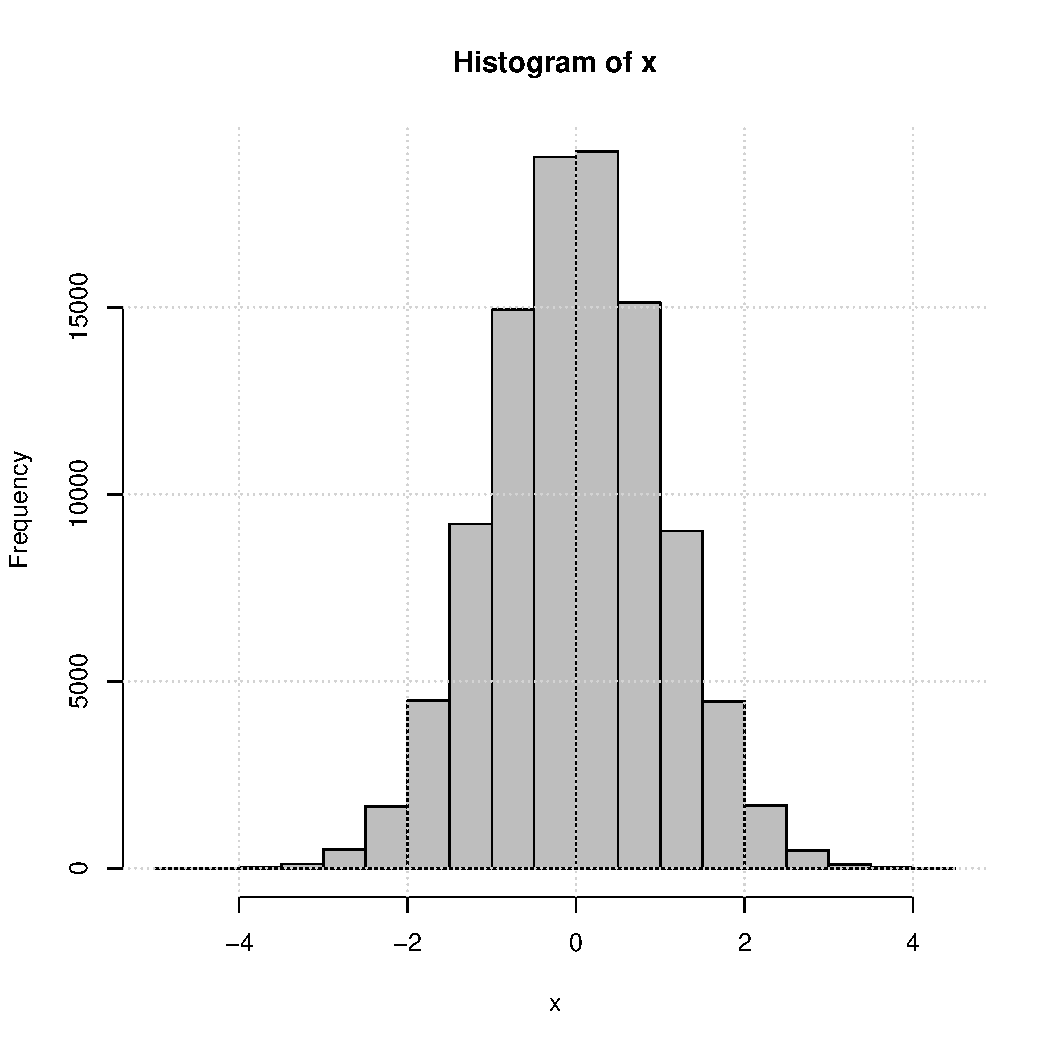
\includegraphics[width=\textwidth]{./figure-1}
  \end{subfigure}

  \captionsetup{margin=10pt,font=small,labelfont=bf,width=.8\textwidth}

  \caption[Krótka nazwa X]{Przykładowy pojedynczy wykres. \textit{Źródło:} opracowanie własne}\label{fig:xxx1}
\end{figure}

\begin{figure}[hbt]
  \centering
  \begin{subfigure}[t]{0.45\textwidth}
    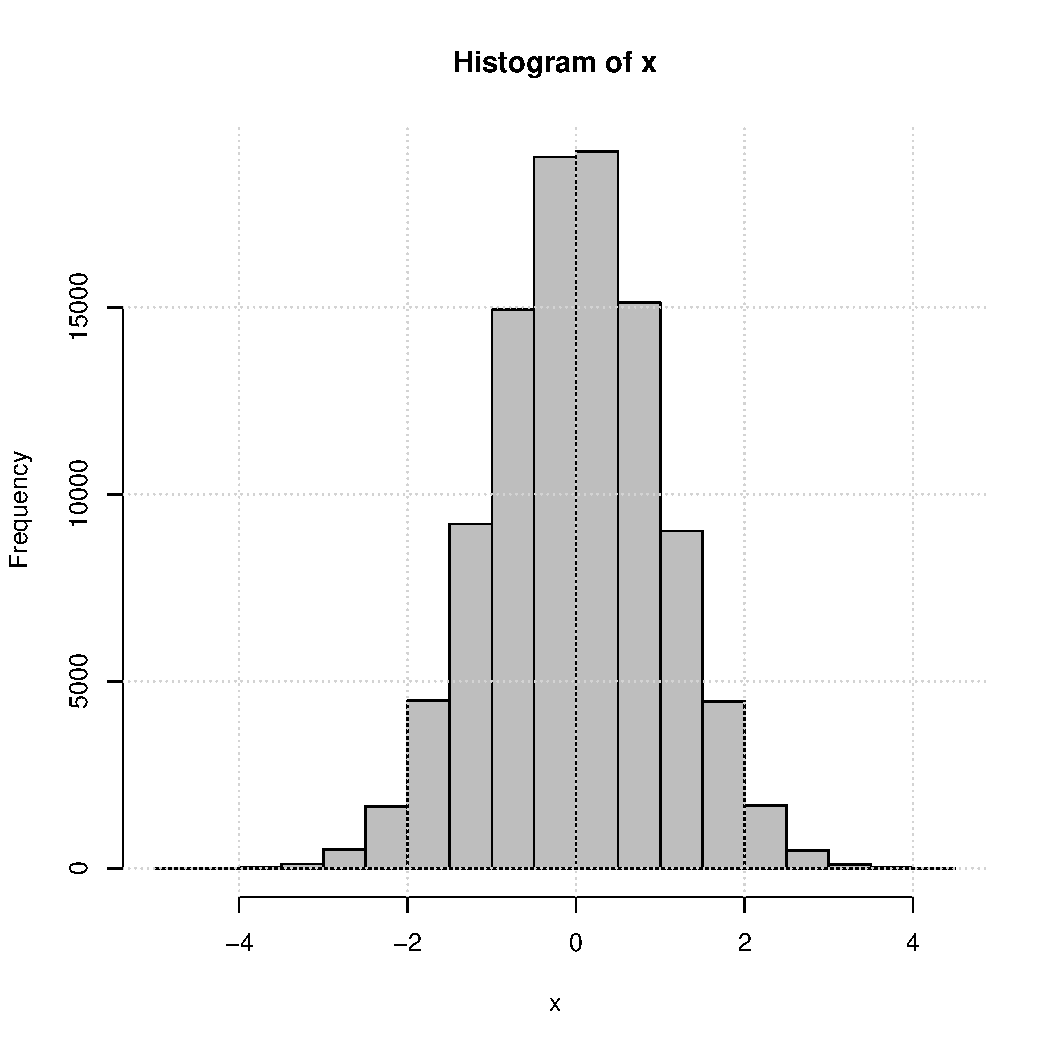
\includegraphics[width=\textwidth]{./figure-1}
    \caption{To jest pierwszy podpis. Ten podpis będzie również zawijany ale będzie to powodowało odpowiednie dopasowanie wysokości.}
    \label{fig:xxxa}
  \end{subfigure}
  \hfill
  \begin{subfigure}[t]{0.45\textwidth}
    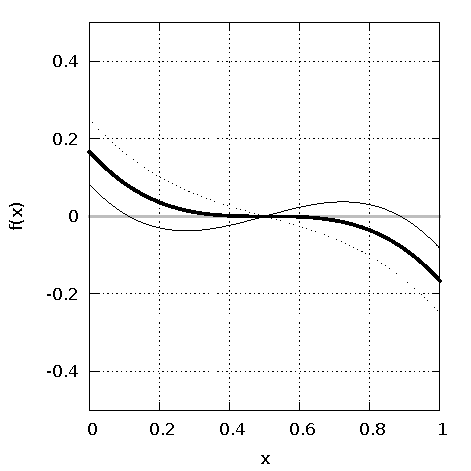
\includegraphics[width=\textwidth]{figure-2}
    \caption{Układ równowag stabilnych}
    \label{fig:xxxb}
  \end{subfigure}

  \captionsetup{margin=10pt,font=small,labelfont=bf,width=.8\textwidth}

  \caption[Krótka nazwa II]{Przykładowy wykres. Wykresy podpisujemy, a więc ten opis znajduje się pod wykresem. \textit{Źródło:} opracowanie własne}\label{fig:xxx}
\end{figure}

Odwołanie się do wykresu działa podobnie jak do równania: rysunek~\ref{fig:xxx1}. Możemy również odwoływać się do podwykresów:~\ref{fig:xxxa} lub \ref{fig:xxxb}. Zarówno tablice (tabele) jak i rysunki (wykresy) są automatycznie układane przez \LaTeX{} i nie pozycjinujemy ich sami.

% --- chapter ---------------------------------------------------------
\clearpage
\section{Literatura}

\begin{wrapfigure}{r}{.5\textwidth}
\centering

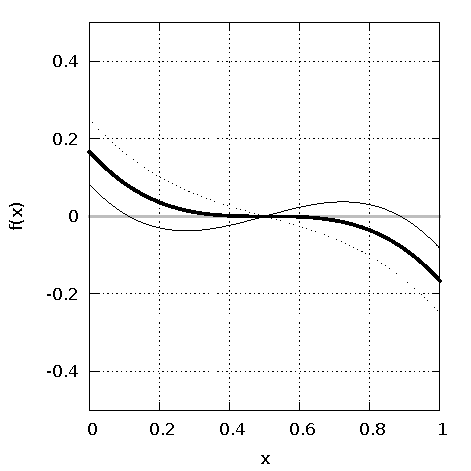
\includegraphics[width=.4\textwidth]{figure-2}

\captionsetup{margin=10pt,font=small,labelfont=bf,width=.42\textwidth}

  \caption[Krótki podpis]{Tak można wstawić wykres opływany tekstem. \textit{Źródło:} opracowanie własne.}\label{fig:yyy}


\end{wrapfigure}


Zawartość literatury znajduje się w innym pliku o nazwie \verb+refs.bib+. Mogą Państwo zmienić nazwę tego pliku ale wtedy trzeba również zmienić w tym pliku informację z \verb+\bibliography{refs}+ na \verb+\bibliography{new-name}+ gdzie \verb+new-name+ jest nazwą nowego pliku z literaturą. Załączony plik  \verb+refs.bib+ zawiera przykłady cytowań dla książek i artykułów.

Sam proces cytowania jest prosty. Używa się komendy \verb+\cite{garland2010}+, która wygeneruje odpowiednie cytowanie \cite{garland2010} oraz dołączy odpowiednią informację na końcu dokumentu.Wszystko jest automatycznie sortowane i formatowane więc nie ma potrzeby zajmowania się tym ręcznie. Przykłady cytowania artykułów z wieloma autorami: \cite{benaim2003}, \cite{osborne1998}.

\begin{longtable}{rrrrr}
\caption{Przykładowe dane}\label{tab:1}                               \\
  \hline
 \( t\) & rok  & wybory & kryzysy & cięcia podatków                   \\ 
  \hline
  \endfirsthead
  \multicolumn{5}{c}%
{\tablename\ \thetable\ -- \textit{kontynuacja z poprzedniej strony}} \\
\hline
\( t\)  & rok  & wybory & kryzysy & cięcia podatków                   \\ 
\hline
\endhead
\hline \multicolumn{5}{r}{\textit{kontynuowane na następnej stronie}} \\
\endfoot
\hline
\endlastfoot
  1     & 1961 & 0      & 0       & 0                                 \\ 
  2     & 1962 & 0      & 0       & 0                                 \\ 
  3     & 1963 & 0      & 0       & 0                                 \\ 
  4     & 1964 & 1      & 0       & 0                                 \\ 
  5     & 1965 & 0      & 0       & 1                                 \\ 
  6     & 1966 & 0      & 0       & 0                                 \\ 
  7     & 1967 & 0      & 0       & 0                                 \\ 
  8     & 1968 & 1      & 0       & 0                                 \\ 
  9     & 1969 & 0      & 0       & 0                                 \\ 
  10    & 1970 & 0      & 0       & 0                                 \\ 
  11    & 1971 & 0      & 0       & 0                                 \\ 
  12    & 1972 & 1      & 0       & 0                                 \\ 
  13    & 1973 & 0      & 0       & 0                                 \\ 
  14    & 1974 & 0      & 1       & 0                                 \\ 
  15    & 1975 & 0      & 1       & 0                                 \\ 
  16    & 1976 & 1      & 0       & 0                                 \\ 
  17    & 1977 & 0      & 0       & 0                                 \\ 
  18    & 1978 & 0      & 0       & 0                                 \\ 
  19    & 1979 & 0      & 0       & 0                                 \\ 
  20    & 1980 & 1      & 0       & 0                                 \\ 
  21    & 1981 & 0      & 0       & 0                                 \\ 
  22    & 1982 & 0      & 1       & 1                                 \\ 
  23    & 1983 & 0      & 0       & 0                                 \\ 
  24    & 1984 & 1      & 0       & 0                                 \\ 
  25    & 1985 & 0      & 0       & 0                                 \\ 
  26    & 1986 & 0      & 0       & 1                                 \\ 
  27    & 1987 & 0      & 0       & 0                                 \\ 
  28    & 1988 & 1      & 0       & 0                                 \\ 
  29    & 1989 & 0      & 0       & 0                                 \\ 
  30    & 1990 & 0      & 0       & 0                                 \\ 
  31    & 1991 & 0      & 1       & 0                                 \\ 
  32    & 1992 & 1      & 0       & 0                                 \\ 
  33    & 1993 & 0      & 0       & 0                                 \\ 
  34    & 1994 & 0      & 0       & 0                                 \\ 
  35    & 1995 & 0      & 0       & 0                                 \\ 
  36    & 1996 & 1      & 0       & 0                                 \\ 
  37    & 1997 & 0      & 0       & 0                                 \\ 
  38    & 1998 & 0      & 0       & 0                                 \\ 
  39    & 1999 & 0      & 0       & 0                                 \\ 
  40    & 2000 & 1      & 0       & 0                                 \\ 
  41    & 2001 & 0      & 1       & 1                                 \\ 
  42    & 2002 & 0      & 0       & 1                                 \\ 
  43    & 2003 & 0      & 0       & 1                                 \\ 
  44    & 2004 & 1      & 0       & 0                                 \\ 
  45    & 2005 & 0      & 0       & 0                                 \\ 
  46    & 2006 & 0      & 0       & 0                                 \\ 
  47    & 2007 & 0      & 0       & 0                                 \\ 
  48    & 2008 & 1      & 1       & 0                                 \\ 
  49    & 2009 & 0      & 1       & 1                                 \\ 
  50    & 2010 & 0      & 0       & 1                                 \\ 
  51    & 2011 & 0      & 0       & 0                                 \\ 
  52    & 2012 & 1      & 0       & 0                                 \\ 
  53    & 2013 & 0      & 0       & 0                                 \\ 
  54    & 2014 & 0      & 0       & 0                                 \\ 
  55    & 2015 & 0      & 0       & 0                                 \\ 
   \hline
\end{longtable}



% --- appendices ------------------------------------------------------
\appendix

% ---------------------------------------------------------------------
\clearpage
\section{Dodatek: Ważne rzeczy do dodania}

Tutaj można włożyć długie tablice, kod wykorzystane w pracy lub inne elementy, które nie powinny zakłócać czytania tekstu.

\begin{landscape}
{\footnotesize
\begin{longtable}{lll}
\caption{Tutaj jest tytuł tablicy}\label{tab:nowatablica1}\\
\hline
Nazwa atrybutu & Wartości & Opis \\ 
\hline
\endfirsthead
\multicolumn{3}{c}%
{\tablename\ \thetable\ -- \textit{kontynuacja z poprzedniej strony}} \\
\hline
Nazwa atrybutu & Wartości & Opis \\
\hline
\endhead
\hline \multicolumn{3}{r}{\textit{kontynuowane na następnej stronie}} \\
\endfoot
\hline
\endlastfoot
chk\_acct & - & stan środków na rachunku bieżącym (jakościowa)\\ 
 & A11 & ... \textless 0 Marek Niemieckich\\  
 & A12 & 0 \textless ... \textless 200 Marek Niemieckich\\  
 & A13 & ... \textgreater 200 Marek Niemieckich\\  
 & A14 & brak rachunku bieżącego\\  
duration & - & czas trwania kredytu w miesiącach (numeryczna)\\  
history & - & przeszłość kredytowa (jakościowa)\\  
 & A30 & brak kredytów w historii/wszystkie kredyty poprawnie spłacone\\  
 & A31 & wszystkie kredyty poprawnie spłacone (zaciągnięte w tym banku)\\  
 & A32 & kredyty poprawnie spłacane po dzień dzisiejszy\\  
 & A33 & opóźnienia w poprzednich spłatach kredytu\\  
 & A34 & konto krytyczne/zaciągnięte kredyty w innych bankach\\  
purpose & - & cel (jakościowa)\\  
 & A40 & nowy samochód\\  
 & A41 & używany samochód\\  
 & A42 & meble\\  
 & A43 & telewizor\\  
 & A44 & urządzenia gospodarstwa domowego\\  
 & A45 & remont\\  
 & A46 & edukacja\\  
 & A47 & wakacje\\  
 & A48 & przekwalifikowanie\\  
 & A49 & biznes\\  
 & A410 & inne\\  
amount & - & kwota kredytu (numeryczna)\\  
say\_acct & - & saldo na rachunku oszczędnościowym/wartość posiadanych obligacji (jakościowa)\\  
 & A61 & ... \textless100 Marek Niemieckich\\  
 & A62 & 100 \textless= ... \textless 500 Marek Niemieckich\\  
 & A63 & 500 \textless= ... \textless 1000 Marek Niemieckich\\  
 & A64 & ... \textgreater= 1000 Marek Niemieckich\\  
 & A65 & nieznane/ brak oszczędności\\  
employment & - & czas zatrudnienia w obecnej pracy (jakościowa)\\  
 & A71 & brak zatrudnienia\\  
 & A72 & ... \textless 1 rok\\  
 & A73 & 1 \textless= ... \textless 4 lata\\  
 & A74 & 4 \textless= ... \textless 7 lat\\  
 & A75 & ... \textgreater= 7 lat\\  
install\_rate & - & wielkość raty jako procent rozporządzalnego przychodu (liczbowa)\\  
pstatus & - & płeć i stan cywilny (jakościowa)\\  
 & A91 & mężczyzna; rozwodnik/w separacji\\  
 & A92 & kobieta; rozwiedziona/ w separacji/ mężatka\\  
 & A93 & mężczyzna ; wolny\\  
 & A94 & mężczyzna ; żonaty/ wdowiec\\  
 & A95 & kobieta ; wolna\\  
other\_debtor & - & inni dłużnicy/ poręczyciele (jakościowa)\\  
 & A101 & brak\\  
 & A102 & współkredytobiorca\\  
 & A103 & poręczyciel\\  
property & - & własność/ mienie (jakościowa)\\  
 & A121 & nieruchomość\\  
 & A122 & (jeśli nie A121) umowa oszczędnościowa/ ubezpieczenie na życie\\  
 & A123 & (jeśli nie A121/A122) samochód lub inne\\  
 & A124 & nieznane\\  
timer\_resid & - & czas zamieszkania w aktualnym miejscu zamieszkania (liczbowa)\\  
age & - & wiek w latach (liczbowa)\\  
other\_install & - & inne zobowiązania ratalne (jakościowa)\\  
 & A141 & bank\\  
 & A142 & sklepy\\  
 & A143 & brak\\  
housing & - & warunki mieszkaniowe (jakościowa)\\  
 & A151 & wynajem\\  
 & A152 & własność\\  
 & A153 & zamieszkanie bez ponoszenia kosztów\\  
other\_credits & - & liczba aktualnych kredytów w tym banku (liczbowa)\\  
job & - & praca (jakościowa)\\  
 & A171 & bezrobotny/niewykwalifikowany; cudzoziemiec\\  
 & A172 & niewykwalifikowany; rezydent\\  
 & A173 & wykwalifikowany pracownik/urzędnik\\  
 & A174 & menadżer/ samozatrudniony/ wysocewykwalifikowany/ wyższy urzędnik\\  
num\_depend & - & liczba osób na utrzymaniu (liczbowa)\\  
telephone & - & telefon (jakościowa)\\  
 & A191 & brak\\  
 & A192 & tak, zarejestrowany pod nazwiskiem klienta\\  
foreign & - & pracownik zagraniczny (jakościowa)\\  
 & A201 & tak\\  
 & A202 & nie\\  
response & - & decyzja kredytowa\\  
 & 1 & tak\\  
 & 2 & nie\\ 
 \hline
\end{longtable}}
\end{landscape}


% --- bibliography ----------------------------------------------------
\clearpage
\bibliographystyle{agsm}
\bibliography{refs}

% --- abstract --------------------------------------------------------
\clearpage
\addcontentsline{toc}{section}{Lista tablic}
\listoftables

% --- abstract --------------------------------------------------------
\clearpage
\addcontentsline{toc}{section}{Lista rysunków}
\listoffigures



% --- abstract --------------------------------------------------------
\clearpage
\addcontentsline{toc}{section}{Streszczenie}
\section*{Streszczenie}

Tutaj zamieszczają Państwo streszczenie pracy. Streszczenie powinno być długości około pół strony.


\end{document}

%%% Local Variables:
%%% mode: latex
%%% TeX-master: t
%%% End:
